\documentclass[a4paper]{spie}  %>>> use this instead for A4 paper

\usepackage[]{graphicx}
\usepackage{cite}

\usepackage{anysize}
\marginsize{3.1cm}{3.1cm}{3.3cm}{4cm}

\title{Experiments on the focusing and use of acoustic energy to accelerate polymer healing} 

\author{Alexander J. Cushman\supit{a}, Brian C. Fehrman\supit{a}, Shaun D. Gruenig\supit{a}, and Umesh A. Korde\supit{a}
\skiplinehalf
\supit{a}South Dakota School of Mines \& Technology, 501 E. St. Joseph St. Rapid City, SD 57701, USA \\
}

\authorinfo{Further author information: (Send correspondence to Umesh A. Korde) \\ U.A.K.: E-mail: umesh.korde@sdsmt.edu, Telephone: 1(605) 394-2401}
 

%%%%%%%%%%%%%%%%%%%%%%%%%%%%%%%%%%%%%%%%%%%%%%%%%%%%%%%%%%%%% 
%>>>> uncomment following for page numbers
% \pagestyle{plain}    
%>>>> uncomment following to start page numbering at 301 
%\setcounter{page}{301} 
 
  \begin{document} 
  \maketitle 

\begin{abstract}
In this paper, we cover our studies on accelerating the molding process of a polymer by applying acoustic stress-wave time reversal. Tests carried out on an epoxy polymer mixed with a curing agent have shown evidence that the introduction of unfocused acoustic energy during the molding process will accelerate that process. The effects of focusing acoustic energy at a mold discontinuity while curing are explored. We also detail our investigations on focusing acoustic energy at a crack location by iteratively applying time reversal. Multiple types of media were tested.
\end{abstract}

%>>>> Include a list of keywords after the abstract 

\keywords{Self healing, Time Reversal, Crack Healing, Polymer Curing}

%%%%%%%%%%%%%%%%%%%%%%%%%%%%%%%%%%%%%%%%%%%%%%%%%%%%%%%%%%%%%
\section{INTRODUCTION}
\label{sec:intro}  % \label{} allows reference to this section
The costs associated with traveling to repair most structures is not a high concern. When it comes to space structures, however, travel becomes a higher concern. Satellites and lightweight space structures are constantly being bombarded by micro-meteoroids and space debris which can cause surface damage in the form of cracks. It is estimated that over 100 billion meteoroids larger than a microgram enter the atmosphere of the Earth everyday. This means that space structures are subject to a high chance of collision with many meteoroids. Damage can also come in the form of impact from space debris. There are over 20,000 trackable space debris objects exceeding a size of 10cm that are in orbit. Surface damage to the structures caused by object impact is nearly inevitable. In addition to high cost and danger of traveling to repair the space structure, there is also the possibility that more space debris will be left behind and further increase the chances of damage to the structures in orbit. For these reasons, it is very desirable to have a structure with the ability to autonomously repair its surface damage. \cite{Close2010, Lee2009}

Self healing materials have been receiving a lot of attention lately. The idea is to apply the biological concept that when a wound occurs the organism will automatically begin to mend itself back together \cite{Scott2011}. One  implementation is to have a material containing two types of micro-capsules that contain either resin or catalyst. When a crack occurs, the two fluids will come into contact and begin the healing process \cite{Mangun2010, White2001, Yuan2008}. The rate of healing needs to occur rather quickly because the crack will attempt to continue expanding while the healing process is taking place. If the rate of crack expansion exceeds the rate of healing then a full recovery may never be achieved.

There are many methods that have been researched in order to speed the rate of recovery. Much of this work has focused on solving the problem from a materials stand point \cite{Sheng2009, Burattini2009, Nakao2009, Fettig2009, Imperiale2009, Zhang2007}. Varying the size of the micro-capsules to maximize the healing rate is one example\cite{Rule2007}. Varying the temperature or exposing the material to ultraviolet light are other examples of ways to speed the healing process \cite{Sloof2009, Song2009, Bosman2009, Djugum2009, Murphy2009, Garcia2009}. Wool and O'Connor have found that the recovery rate can be accelerated by increasing the pressure at the recovery site and more recent work supports this concept \cite{Wool1981, Sharma2011}. We wish to apply acoustic stress waves to increase the localized pressure at a healing site and, in turn, increase the rate at which the material recovers. 

It would be inefficient to blindly send acoustic energy throughout the system in a continuous fashion whether or not damage has occurred. Not only will this unnecessarily consume a large amount of power, it also has the potential to resonant within the structure and cause damage. Therefore, it is desirable to have a system that is able to detect when damage occurs and then begins to focus acoustic energy at that damaged location. This focusing would be done without actual knowledge of the crack's location. Acoustic time reversal is one such method that could be used. Many variations and applications of time reversal have been studied \cite{Anderson2008, Anderson2009, Ambrozinski2012, Borcea2003, Dahl2009, Fink2009, Foroozan2011, Harley2009, Sinelnikov2010, Sutin2004}. One method is to iteratively apply time reversal such that a better focusing of the acoustic energy at a crack location is achieved with each iteration.

In this paper we detail our latest studies on using acoustic energy to accelerate epoxy curing. We have performed more tests using a two-part epoxy. These tests involve monitoring the curing rate of the epoxy with and without acoustic energy being introduced to see if there is an effect. Iterative time reversal has also been carried out on both dispersive and non-dispersive rods. The goal of the time reversal was to focus energy and increase the response amplitude at a ``defect'' location within the rod system over a number of iterations.

%%%%%%%%%%%%%%%%%%%%%%%%%
\section{Experimental Implications}
\label{sec:exp_imp}
We have broken the overall project into two main components for us to study. The first component is determining the relationship between acoustic excitation and the curing rate of a self healing material. Wool and O'Connor have also shown that the processes of a self healing material mending itself and an epoxy curing can be treated the same. This is due to the fact that both substances will traverse the same five steps during their curing process which are: (i) surface rearrangement, (ii) surface approach, (iii) wetting, (iv) diffusion, and (v) randomization. Experimentally, we look at the curing process of a two part epoxy with and without excitation from a speaker. 

Focusing of acoustic energy is the second component of the project. It is needed to efficiently increase the healing rate at a crack location. Time reversal experiments have been carried out using new setups involving multiple types of media. These tests are used to determine the effectiveness of the time reversal algorithm in focusing the energy of the acoustic waves.

%%%%%%%%%%%%%%%%%%%%%%%
\subsection{Epoxy Curing Experiments}

Over the last two years, the epoxy curing project's setup and experiments have remained mostly unaltered. A two-part epoxy is used to fill a brass tube and the curing process is then monitored. To monitor this process, two sensors are used: a thermistor which rests inside the curing epoxy to provide temperature feedback, and an accelerometer attached to the brass tube to record a vibrational response. These vibrations are generated by a marble dropper which is positioned over the tube. We plot the FFTs of these vibrational responses and use them to characterize the state of the cure process. The idea is that the response will change as the epoxy cures. This setup is kept in a temperature-controlled container, which provides more consistent results. Using the LabVIEW programming environment, new software has been made for acquiring data which allows more reliable testing and easier data manipulation. New hardware is also being used which gives greater control over the data acquisition process. 

In these experiments, we compare the rate of curing with and without acoustic excitation. This excitation is created using a simple setup: a speaker is placed on top the box which houses the experiment.
Figures \ref{fig:epoxy_rod} and \ref{fig:speaker} show the experiment's current configuration(without the marble dropper or container).

\begin{figure}[h!]
\begin{center}
\begin{tabular}{c}
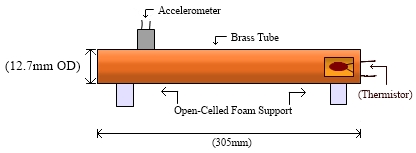
\includegraphics[height=5.5cm]{epoxy_rod}
 \end{tabular}
\end{center}
\caption[example] 
%>>>> use \label inside caption to get Fig. number with \ref{}
{ \label{fig:epoxy_rod} 
   The dimensions and setup for experiment which monitors the curing process of the epoxy without the use of acoustic excitation
   }
\end{figure} 
   
 \begin{figure}[h!]
\begin{center}
\begin{tabular}{c}
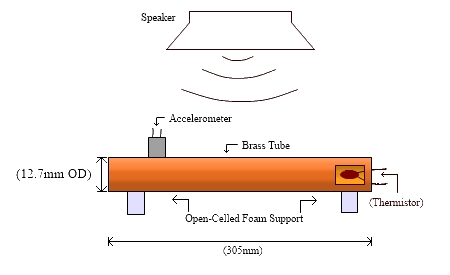
\includegraphics[height=8.5cm]{speaker}
\end{tabular}
\end{center}
\caption[example] 
%>>>> use \label inside caption to get Fig. number with \ref{}
{ \label{fig:speaker} 
   The dimensions and setup for experiment which monitors the curing process of the epoxy. This time, however, acoustic energy is being introduced into the system.
   }
\end{figure} 

%%%%%%%%%%%%%%%%%%%%
\subsection{Iterative Time Reversal Experiments}
The idea is to focus acoustic wave energy at a crack location within a system. For these experiments, we use a system of solid, circular rod segments. Ultrasonic waves are propagated through these rods using ceramic piezoelectric transducers (PZTs). These same transducers are also able to acquire signals based on their response to acoustic excitation. Two rod segments are used in these experiments. A PZT is sandwiched between the ends of these two rods in order to form a ``crack'' in the system and also read the response at that point. We will refer to this as the crack PZT. A PZT is then placed on each open end of the system and everything is compressed. We will refer to these end PZTs as Ch0 and Ch1. This system is shown in Figure \ref{fig:steel_rods}.

\begin{figure}[h!]
\begin{center}
\begin{tabular}{c}
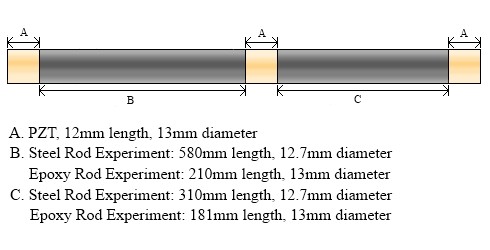
\includegraphics[height=8.5cm]{steel_rods}
\end{tabular}
\end{center}
\caption[example] 
%>>>> use \label inside caption to get Fig. number with \ref{}
{ \label{fig:steel_rods} 
   Overview of the setup and dimensions for the iterative time reversal experiments}
\end{figure} 

One of these end PZTs (Ch0, for this example) will send a short signal through the rod system. When this signal reaches the crack PZT, part of its energy will reflect back to the sending PZT (Ch0) and part will continue propagating to the PZT on the opposite end of the system (Ch1). If the end PZTs  (Ch0 and Ch1) capture, amplify, and replay these waves in a time reversed fashion, then they will recombine at the location where they split. This location is the site of the crack PZT and we will achieve a focusing of energy at that location. This process is then applied iteratively. With each iteration we see a better focusing of the waves and an increase in amplitude at the crack PZT. The gains eventually level off and we considering the algorithm has having converged. Between each iteration, we also introduce a delay time. This allows for the residual vibrations in the system to die down. Waiting for the ringing to subside will help to prevent the system from resonating and becoming damaged.

These tests were carried out using two different types of rods. The first were a set of steel rods. These provided a nice transmission of the waves and eased the analysis. The other set of rods tested were brass rods filled with epoxy. This epoxy has been left to fully cure before testing of the time reversal algorithm. These brass rods proved to be much more dispersive than the steel rods. Due to this reason, a slightly different method of time reversal was used for these experiments than what was described above. Both time reversal algorithms are detailed in Figure \ref{fig:flow_chart}.

\begin{figure}[h!]
\begin{center}
\begin{tabular}{c}
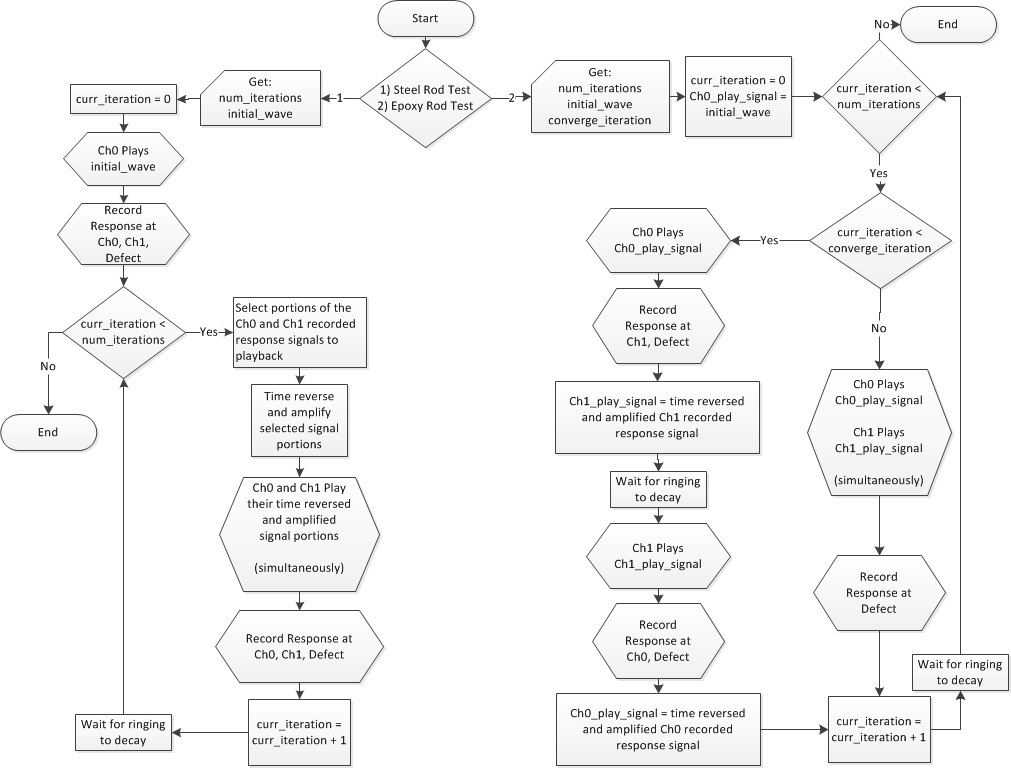
\includegraphics[height=10cm]{flow_chart}
\end{tabular}
\end{center}
\caption[example] 
%>>>> use \label inside caption to get Fig. number with \ref{}
   { \label{fig:flow_chart} 
   Flowchart detailing the iterative time reversal algorithms used for each rod system, with the algorithms differing just slightly between the steel rods and the epoxy-filled brass rods}
\end{figure} 

%%%%%%%%%%%%%%%%
\section{Experimental Results}

%%%%%%%%%%%%%
\subsection{Results of Epoxy Curing}
After using the accelerometer to record the vibrational response from the collisions of the marbles with the brass tube as previously discussed, we are able to plot the FFT of this response. As the curing process elapses, the frequencies that the epoxy has the greatest response to will shift, as seen in Figure \ref{fig:fft1}. This figure also shows that the amplitudes of these peaks shift as well. Comparing the peaks on the FFT plot at any given point in the curing process to the peaks on the FFT plot of the fully cured sample is used to determine the progress of the curing process at that point. This is used to compare the curing rate of the epoxy with and without acoustic excitation. Figure \ref{fig:fft1} shows one such FFT plot, where the lighter plot shows the vibrational response of the epoxy without acoustic excitation after two hours and the darker plot shows the response after the epoxy has fully cured. Figure \ref{fig:fft2} shows the same FFT plots, but with the introduction of acoustic energy to the system. As shown by these plots, it appears that the acoustic energy introduced succeeds in accelerating the curing process of the epoxy.

\begin{figure}[h!]
\begin{center}
\begin{tabular}{c}
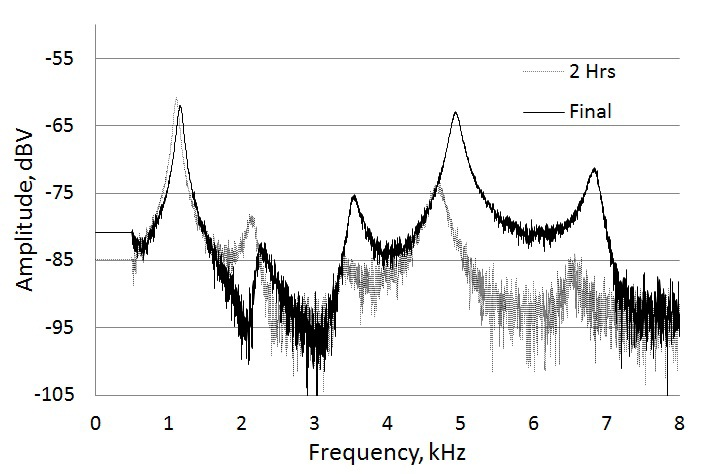
\includegraphics[height=8.5cm]{fft1}
\end{tabular}
\end{center}
\caption[example] 
%>>>> use \label inside caption to get Fig. number with \ref{}
{ \label{fig:fft1} 
   FFT of the vibrational response at 2 hours and 24 hours of the curing process for the epoxy-filled brass rod without acoustic excitation.}
\end{figure} 
   
\begin{figure}[h!]
\begin{center}
\begin{tabular}{c}
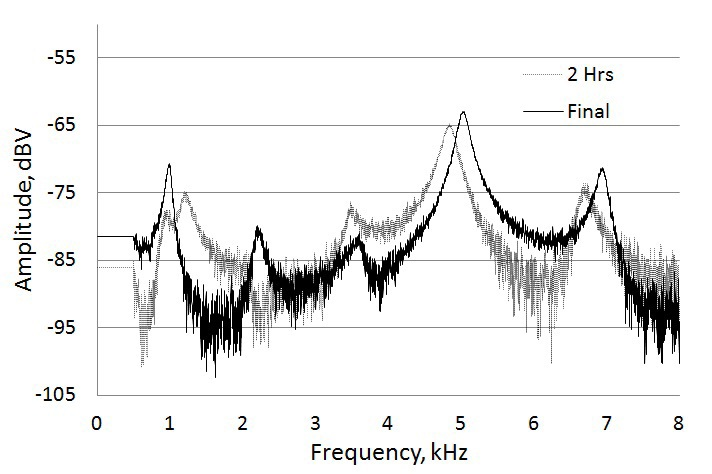
\includegraphics[height=8.5cm]{fft2}
\end{tabular}
\end{center}
\caption[example] 
%>>>> use \label inside caption to get Fig. number with \ref{}
{ \label{fig:fft2} 
   FFT of the vibrational response at 2 hours and 24 hours of the curing process for the epoxy-filled brass rod with acoustic excitation being introduced.}	
\end{figure}

%%%%%%%%%%%%%%%%%%%
\subsection{Results of Iterative Time Reversal}
The iterative time reversal produced fairly good results for both rod system. With both the steel and the epoxy-filled brass rods we were able to get an increased response amplitude at the crack PZT location. Figure \ref{fig:steel_tr} shows the results for the experiment performed on the steel rod system. Six iterations are plotted. The response produced at the crack PZT is seen to be considerably higher on the final iteration than on previous iterations.

\begin{figure}[h!]
\begin{center}
\begin{tabular}{c}
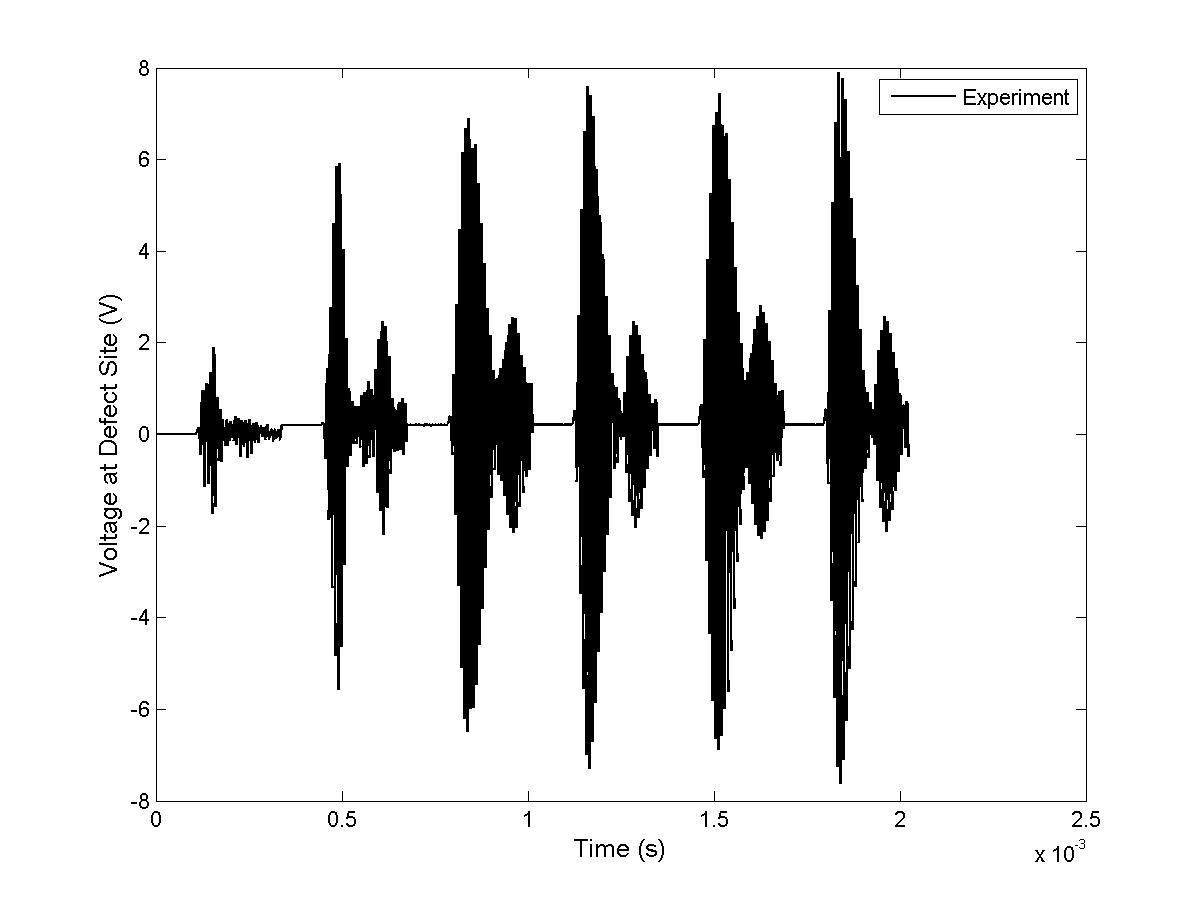
\includegraphics[height=8.5cm]{steel_tr}
\end{tabular}
\end{center}
\caption[example] 
%>>>> use \label inside caption to get Fig. number with \ref{}
 { \label{fig:steel_tr} 
   Graph which shows the response at the crack PZT for the steel rod system when using the iterative time reversal algorithm. Multiple iterations are plotted. With each iteration, the amplitude of the response increases. Secondary waves are thought to result from the adhesive which is used to better the rods and PZTs. This is being investigated in newer systems.
}
\end{figure} 
   
Analysis was performed in order to predict the response at the crack PZT. This was compared to experimental data. A reasonable match is seen between the two. This is shown in Figure \ref{fig:steel_theory_exp}.


\begin{figure}[h!]
\begin{center}
\begin{tabular}{c}
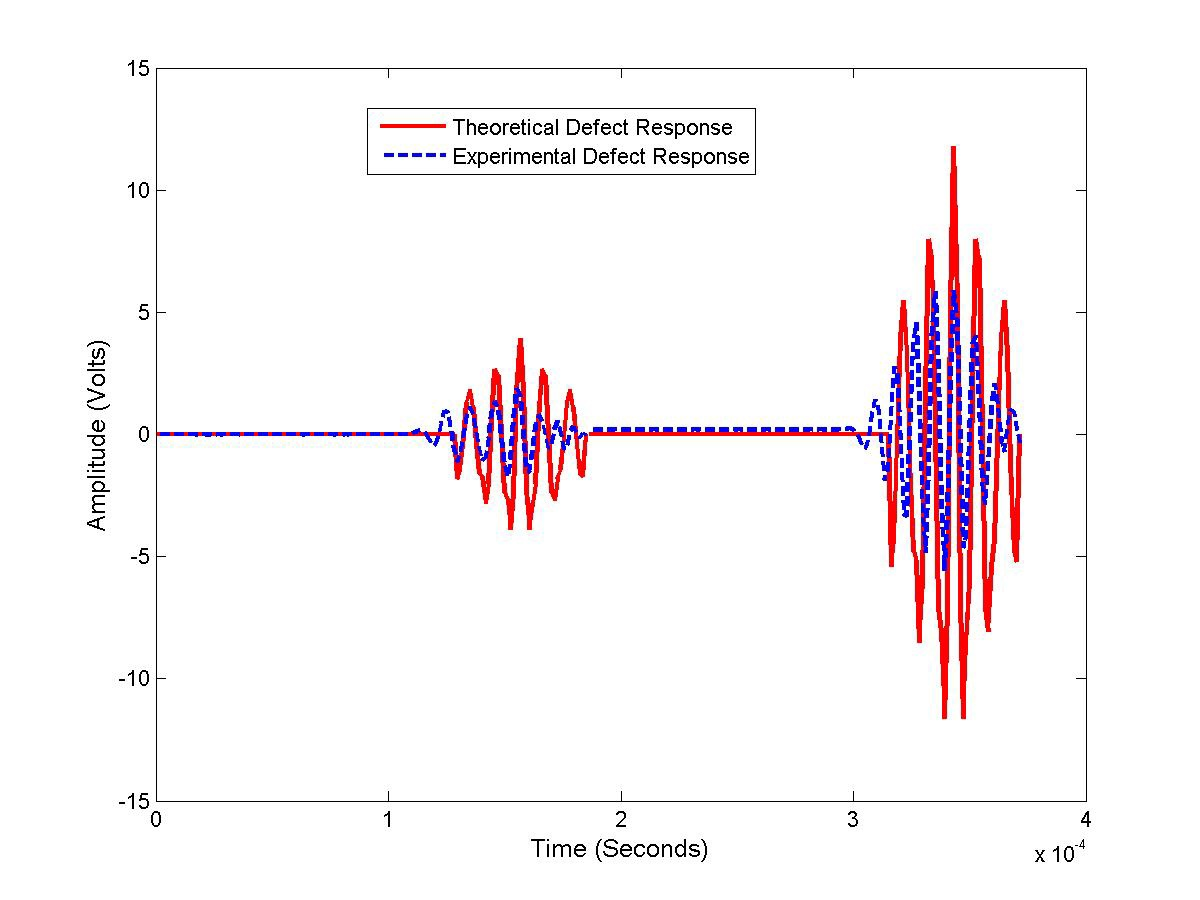
\includegraphics[height=8.5cm]{steel_theory_exp}
\end{tabular}
\end{center}
\caption[example] 
%>>>> use \label inside caption to get Fig. number with \ref{}
{ \label{fig:steel_theory_exp} 
   Shows the comparison between the predicted and the experimental response at the defect location. The secondary waves seen in the early graph have been omitted.
}
\end{figure} 
   
Results similar to those seen with the steel rods were obtained in the epoxy-filled brass tube experiments. We see an increased response at the crack PZT as the iterations of the time reversal progress. Even with the high dispersion of the epoxy, we are still able to achieve a level of focusing at a point within the system. The results of the epoxy rod tests can be viewed in Figure \ref{fig:epoxy_tr}.

\begin{figure}[h!]
\begin{center}
\begin{tabular}{c}
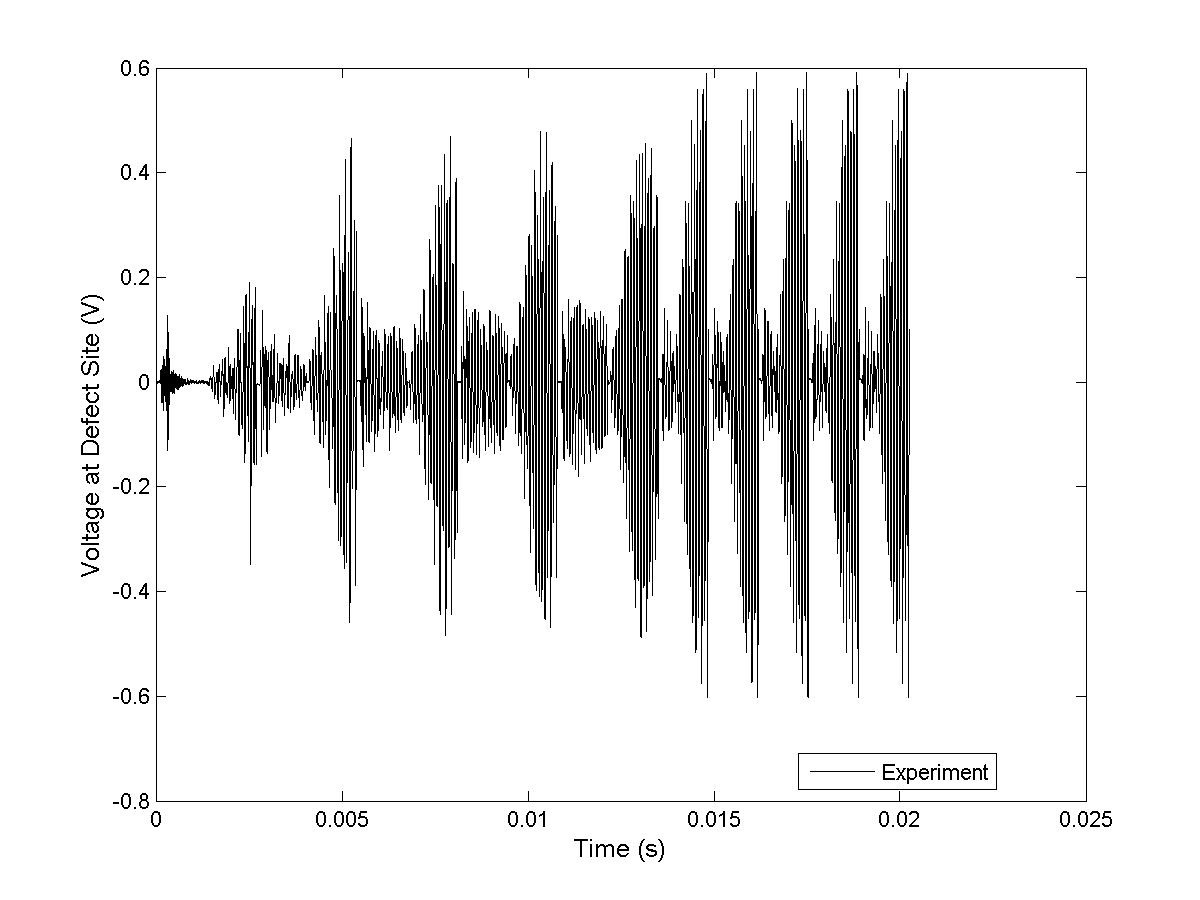
\includegraphics[height=8.5cm]{epoxy_tr}
\end{tabular}
\end{center}
\caption[example] 
%>>>> use \label inside caption to get Fig. number with \ref{}
{ \label{fig:epoxy_tr} 
   Amplitude of the response at the crack PZT for multiple iterations of the time reversal algorithm. The amplitude appears to increase throughout the iterations.
}
\end{figure} 


%%%%%%%%%%%%%%%%%%%%%%%%%%%%
\section{Conclusions and Future Work}
The results of our epoxy experiments suggest that the presence of acoustic energy will accelerate the curing process of the epoxy. There is a strong evidence from the time reversal experiments that we can increase the pressure at a crack location by focusing acoustic waves at that point. If we apply the time reversal iteratively then we are able to achieve an even better focusing at the crack site. Analytical results have a decent match to the experimental results for the steel rod tests. Both dispersive and non-dispersive media were tested and both showed good results. Future tests will involve further verification of the affects of acoustic energy on epoxy curing. We will also attempt to use iterative time reversal in order to fuse nylon rod segments together. Tests will also be carried out which will put the epoxy curing and time reversal experiments together in order to enhance the curing speed of the epoxy.

%%%%%%%%%%%%%%%%%%%%%%%%%%%%%%%%%%%%%%%%%%%%%%%%%%%%%%%%%%%%%
\acknowledgments     %>>>> equivalent to \section*{ACKNOWLEDGMENTS}       
 
We would like to thank the Air Force Research Laboratory for their continued support and also acknowledge Joe Harley and his team from Carnegie Mellon for their input on the project. 

%%%%%%%%%%%%%%%%%%%%%%%%%%%%%%%%%%%%%%%%%%%%%%%%%%%%%%%%%%%%%
%%%%% References %%%%%

\bibliography{references}   %>>>> bibliography data in report.bib
\bibliographystyle{spiebib}   %>>>> makes bibtex use spiebib.bst

\end{document} 
